\documentclass{article}
\usepackage{amsmath, amssymb}
\usepackage{amsfonts} 
\usepackage{graphicx}
\usepackage[a4paper, total={6.4in, 9.5in}]{geometry}
\usepackage{hyperref}
\usepackage{authblk}
\usepackage[utf8]{inputenc}

\usepackage{xcolor}
\usepackage{mdframed}

\usepackage{multirow}

\makeatletter
\DeclareRobustCommand*{\Myhref}[1][]{% definition copied form hyperref.sty
  \begingroup
  \setkeys{Hyp}{#1}% Changed href to Hyp
  \@ifnextchar\bgroup\Hy@href{\hyper@normalise\href@}%
}
\makeatother

\newtheorem{theorem}{Theorem}

\begin{document}

\title{Public key encryption for pedestrians: \\ RSA + OAEP padding with a real SSH key}

\author{Laurent Bou\'e \\ \Myhref[hidelinks]{mailto:ranlot75@gmail.com}{\protect
\includegraphics[width=1cm,height=0.6cm]{logos/gmail.png}} \,\,\,\, \Myhref[hidelinks]{https://www.linkedin.com/in/laurent-bou\%C3\%A9-b7923853/}{\protect
\includegraphics[width=0.8cm,height=0.8cm]{logos/linkedin.png}} \,\,\,\, \Myhref[hidelinks]{https://github.com/Ranlot}{\protect
\includegraphics[width=1cm,height=1cm]{logos/github.png}} \,\,\,\, \Myhref[hidelinks]{https://twitter.com/ranlot75}{\protect
\includegraphics[width=0.8cm,height=0.8cm]{logos/twitter.png}} }
\affil{Microsoft}
\date{}

\maketitle

\begin{abstract}
The purpose of these notes is to provide an introduction to the RSA public key encryption algorithm.  It is meant to be read as a formal support to an accompanying interactive~\texttt{Jupyter notebook} where all the steps are illustrated end-to-end.  Unlike many other tutorials, the notebook is based on a real-world SSH key pair generated by~\texttt{ssh-keygen}.  Finally, we go beyond textbook RSA and its homomorphic properties by introducing the~OAEP padding scheme.
\end{abstract}

\vspace{0.5cm}

\begin{mdframed}[backgroundcolor=yellow!20] 
{\bf Online resources.} \href{https://github.com/Ranlot/public-key-encryption}{All source code including the companion~\texttt{Jupyter notebook} and even more cryptograhy notebooks are available on GitHub @ \texttt{https://github.com/Ranlot/public-key-encryption}}
\end{mdframed}

\vspace{0.2cm}

\section{Textbook RSA}
\label{sec::algo}

Instead of introducing cryptosystems from a historical perspective and discussing how public key encryption underpins many core digital communication systems that we take for granted (plenty of \href{https://en.wikipedia.org/wiki/RSA_(cryptosystem)}{material} can be found easily online), we delve right into a more technical description.  The original paper~\cite{rsaOriginal} is easily readable and should serve as the first point of reference.  Procedurally, the RSA~algorithm goes as follows:
\begin{itemize}
\item Pick two random primes~$p \neq q$.  For example, in the \href{https://github.com/Ranlot/public-key-encryption}{accompanying \texttt{Jupyter notebook}},~$p$ and~$q$ are are generated by~\texttt{ssh-keygen} and have both~$b=1024$ bits.  The question of how many such~$b$-bit primes exist, how to find them and more generally of the scale of the numbers involved is addressed at the end of this section.
\item Next, calculate two other integers
\begin{itemize}
    \item the product~$n=p \cdot q$ which will be referred to as the ``public modulus''.  Continuing with our \href{https://github.com/Ranlot/public-key-encryption}{\texttt{Jupyter notebook}} where~$p$ and~$q$ are both composed of~$b=1024$ bits, their product has~$2b = 2048$ bits and the cryptosystem is referred to as~RSA-2048~\footnote{Although RSA-2048 is still the default modulus for \texttt{ssh-keygen}, it is recommended to use RSA-4096 and improve the level of security.  Other than choosing larger random primes~$p$ and~$q$ with~2048 bits so that the public modulus~$n$ has~$4096$~bits, there is no procedural and/or conceptual difference with the generic algorihtm presented in these notes.}.  
    \item the Euler's totient function~$\varphi(n)$ associated with the public modulus.  In general,~$\varphi(n)$ counts the number of integers less than~$n$ that are coprimes with~$n$.  Because~$p$ and~$q$ are primes,~$\varphi(n)$ can also be expressed as a product
    \begin{equation}
        \varphi(n) = \varphi(p\cdot q) = \varphi(p) \cdot \varphi(q) \quad \rightarrow \quad \varphi(n) = (p-1) \cdot (q-1)
    \label{eq:totient}
    \end{equation}
    as can be \href{https://en.wikipedia.org/wiki/Euler's_totient_function}{shown} by applying the Chinese remainder theorem.  Furthermore, since prime numbers cannot be factorized, it is clear that~$\varphi(p) = p-1$ and~$\varphi(q) = q-1$.
\end{itemize}
\item Next, we choose the ``public exponent'' as a (potentially random) number~$e$ coprime with the~$\varphi(n)$ evaluated in the previous step.  In practice~$e$ is not random, it is usually fixed to~$e = 2^{16} + 1 = 65537$ and one should verify that~$\text{gcd}(e, \varphi(n)) = 1$ so that the coprimality condition is satisfied.
\item Now that we have~$\varphi(n)$ and~$e$, we define the ``private exponent''~$d$ as the modular inverse of~$e$ with respect to the modulo~$\varphi(n)$ so that
\begin{equation}
e \cdot d \equiv 1 \,\,\text{mod}\,\, \varphi(n)
\label{eq:privateExp}
\end{equation}
Since the public exponent~$e$ was chosen to be coprime with~$\varphi(n)$, the private exponent~$d$ is guaranteed to exist and be unique.  It can be found efficiently using Euclid's extended algorithm (see \hyperlink{theorem1}{Theorem~1}).
\item At this point, the RSA key generation process is complete
\begin{itemize}
    \item public key: composed of the modulus and the public exponent~$(n, e)$.
    \item private key: simply the private exponent~$d$.  Note that the original two primes~$p, q$ and~$\varphi(n)$ should not be shared publicly since they can be used to recover~$d$.
\end{itemize}
\item Encryption.  Given a plaintext~$m$ (converted to an integer in a process that will be illustrated in section~\ref{sec::example}) and the public key~$(n, e)$, the encrypted cipher~$c$ is obtained by raising~$m$ to the public exponent~$e$ and keeping only its remainder after division with the public modulus~$n$.  In other words, the encryption function~$\mathcal{E}$ is given by the modular exponentiation
\begin{equation}
c \equiv \mathcal{E}(m) \equiv m^e \,\,\text{mod}\,\,n
\label{eq::RSA_encrypt}
\end{equation}
The plaintext message should never exceed~$n$ otherwise we lose uniqueness.  If we are in a situation where~$m > n$, the message should be split into multiple messages that are all smaller than~$n$.
\item Decryption.  Given the ciphertext~$c$ and the private key~$d$, the original message is recovered by another modular exponentiation
\begin{equation}
\mathcal{D}(c) \equiv  c^d \,\,\text{mod}\,\,n 
\label{eq::RSA_decrypt}
\end{equation}
In section~\ref{sec:certification}, we will prove that the decryption function~$\mathcal{D}$ always recovers the original plaintext message
\begin{equation*}
\mathcal{D}(c) \equiv \mathcal{D} \left( \mathcal{E}(m) \right) \equiv m \,\,\text{mod}\,\,n
\end{equation*}
\end{itemize}

\paragraph{What's the trick?}  Informally, encryption consists in raising the message to the power~$e$.  Decryption promptly reverses the effect of encryption by raising the ciphertext to the inverse power~$d \sim e^{-1}$.  Obviously, modular arithmetic with respect to~$\varphi(n)$ introduces more complexity.  Nevertheless, the crux of the problem stems from the fact calculating~$\varphi(n)$ itself turns out to be a computationally infeasible task.  In fact, it can be shown that evaluating~$\varphi(n)$ is equivalent to factorizing~$n = p\cdot q$ into its primes; a deceivingly difficult \href{https://en.wikipedia.org/wiki/Integer_factorization}{problem} for which there is no known efficient classical algorithm (see~\cite{RSAquantum} for implementations of \href{https://en.wikipedia.org/wiki/Shor\%27s_algorithm}{Shor's algorithm} on the current generation of quantum computers).  In other words, unless someone was told the values of~$p$ and~$q$, in which case it would be trivial to calculate~$\varphi(n)$ using~eq.(\ref{eq:totient}) and immediately determine the private exponent~$d$ using~eq.(\ref{eq:privateExp}) and Euclid's extended algorithm (see \hyperlink{theorem1}{Theorem~1}), there is no known feasible computation that can yield the private exponent (without knowing~$p$ and~$q$ to begin with).  Functions that are easy to calculate in one direction but hard to invert (without special information) are known as ``trapdoor'' functions.  For RSA, it is prime factorization that is used as the trapdoor function.  Other cryptosystems may be based on different trapdoor functions not based on number theory but rather on geometry and discrete logarithms in the case of \href{https://en.wikipedia.org/wiki/Elliptic-curve_cryptography}{elliptic curve cryptography} or on \href{https://en.wikipedia.org/wiki/Lattice-based_cryptography}{lattice-based} problems in the case of more modern quantum-resistant cryptographic primitives.  We refer the reader to~\cite{sigmaprime} for an excellent discussion of why Euler's totient function~$\varphi$ naturally comes up as the simplest candidate to construct a non-trivial encryption/decryption scheme.

\paragraph{Getting a feel for the size of the numbers in question}  In case one was thinking about trying to brute-force factorize~$n$, it is interesting to get a feeling for the size of numbers in question.  We will do this by asking a few questions about~$b$-bit numbers and applying the solutions to~RSA-2048.
\begin{itemize}
\item[--] How many~$b$-bit numbers are there?  In order to have exactly~$b$ bits (no more and no less) all numbers have to start with~1 as the leading bit.  Since the remaining~$b-1$ bits can take all possible values, there are~$2^{b-1}$ numbers with exactly~$b$ bits.  With~$b=1024$ bits, this translates into~$2^{1023} \approx 9 \times 10^{307}$ possible numbers.
\item[--] How many of these are prime?  According to the \href{https://en.wikipedia.org/wiki/Prime_number_theorem}{prime number theorem}, the number of primes~$\pi(x)$ less than or equal to~$x$ converges to~$\lim_{x \rightarrow \infty} \pi(x) = x / \log x$.  Therefore the number of primes with exactly~$b$ bits can be estimated as~$\pi ( 2^b )  - \pi ( 2^{b-1} ) \approx 2^{b-1} / (b \log 2)$ which is a small fraction of the total number of numbers~$2^{b-1}$.  With~$b=1024$ bits, this still leaves a staggering~$\approx 1.3 \times 10^{305}$ (about~$0.14\%$ of all~1024-bit numbers) possibilities from which we can choose the random primes~$p$ and~$q$.
\item [--] What is the average value of a random~$b$-bit number?  As the leading bit must always be~1 it will always contribute~$2^{b-1}$ to the average value.  Assuming that the remaining~$b-1$ bits are successfully distributed uniformly and independently of each other, their contribution to the average value is given by~$\sum_{k=0}^{2^{b-1}-1} k / \, 2^{b-1} \approx 2^{b-2}$.  Summing up both terms we find that the average value of a~$b$-bit number is~$\approx 3 \times 2^{b-2}$.  For random primes~$p$ and~$q$ with~$b = 1024$, this translates into~$p \sim q \sim 10^{308}$.  The public modulus with~$2b = 2048$ bits can be expected to be on the order of~$n \sim 10^{616}$.
\item [--] How to find the random primes~$p$ and~$q$?  Unlike integer factorization, primality testing is relatively ``easy'' (polynomial time with the size of the numbers being tested and the allowed error rate).  Although Fermat's little theorem (see \hyperlink{theorem2}{Theorem~2}) could be used as a simple probabilistic test of compositeness, stronger algorithms such as the \href{https://en.wikipedia.org/wiki/Miller\%E2\%80\%93Rabin_primality_test}{Miller-Rabin test} are used in real-world systems such as~\texttt{ssh-keygen}. Since about one out of every~$\log n$ numbers around~$n$ is prime (see the prime number theorem above), this means that we only need to test about~$\log 10^{616} \sim 1400$~random integers before a prime is found (very rough estimation, of course) for~RSA-2048.
\end{itemize}

\noindent Now that we have a better idea for the scale of the numbers in question, we can go back to the idea of a brute-force attack.  One of the most na\"ive approach would be to generate a lot of pairs~$(p_\text{test}, q_\text{test})$ and look for a match between one of our~$n_\text{test} = p_\text{test} \cdot q_\text{test}$ with another publicly available~$n_\text{target}$ for which we wish to extract the private key. After generating a million~$\sim 10^{6}$ primes, we have~$\sim 10^{12}$ possible~$n_\text{test}$'s for which we know the factors.  Storing this information already takes up a questionable~$\sim 384 \, \text{TB}$ since we need to keep at least one~$1024$-bit factor (either~$p_\text{test}$ or~$q_\text{test}$) and the corresponding~$2048$-bit modulus~$n_\text{test}$.  Unfortunately, all this data gives us only a~$\sim 10^{-604}$ probability that we were able to generate a collision.  Pushing this idea to the absurd and assuming that we could get our hands on~$\sim 10^{80}$ distinct random primes ($\sim$~\href{https://en.wikipedia.org/wiki/Observable_universe#Matter_content_\%E2\%80\%93_number_of_atoms}{number of atoms in the universe}) would only increase our probability of finding a colliding public modulus to~$10^{-456}$...  More realistic attack vectors and how to secure RSA against them by introducing randomized padding will take us away from textbook RSA in section~\ref{sec::padding}.

\paragraph{\href{https://en.wikipedia.org/wiki/Digital_signature}{Digital signature}}  Since~$e$ and~$d$ are modular inverses of each other, we have~$m\equiv (m^e)^d \equiv (m^d)^e \,\,\text{mod}\,\,n$.  In other words, it is possible to invert the purpose of each key: encrypt a message with the private key and decrypt with the public key.  By appending the private-key-encrypted version of a message and sending this signature along with the plaintext message, free for all to see, any recipient with the public key can verify the authenticity and integrity of the message.  Digital signatures are \href{https://github.com/Ranlot/public-key-encryption}{illustrated in the~\texttt{Jupyter notebook}} and follow exactly the same logic simply flip-flopping between private and public keys.

\section{Correctness of the decryption}
\label{sec:certification}

Why does the decryption function~$\mathcal{D}(c)$ applied to a cipher~$c = \mathcal{E}(m)$ always take us back to the original plaintext message~$m$?  After following a na\"ive proof strategy which achieves a (very convincing) probabilistic statement, we delve into a complete proof and finish by showing how to optimize the decryption process.

\subsection{Probabilistic ``proof''}
\label{sec::probaProof}

\noindent Let us start with a na\"ive strategy and propose to evaluate~$\mathcal{D}(c)$ in the most straightforward way possible
\begin{align*}
\mathcal{D}(c) &\equiv c^d \,\,\text{mod}\,\,n \\
&\equiv (m^e)^d \,\,\text{mod}\,\,n \\
&\equiv m^{e d} \,\,\text{mod}\,\,n
\end{align*}
where we replaced the cipher~$c$ by its expression defined in~eq.(\ref{eq::RSA_encrypt}).  At this point, we remember that the private exponent~$d$ is defined as the modular inverse of the public exponent~$e$. Re-writing~eq.(\ref{eq:privateExp}) by introducing an integer~$k \in \mathbb{Z}$ to make the congruence explicit yields
\begin{equation*}
e \cdot d = 1 + k \cdot \varphi(n)
\end{equation*}
allowing us to continue evaluating~$\mathcal{D}(c)$ as
\begin{align*}
\mathcal{D}(c) &\equiv m^{1 + k \varphi(n)} \,\,\text{mod}\,\,n \\
&\equiv m \, (m^{\varphi(n)})^k \,\,\text{mod}\,\,n \\
&\equiv m \, \underbrace{\big( m^{\varphi(n)} \times \cdots \times m^{\varphi(n)}}_{k \, \text{times}} \big) \,\,\text{mod}\,\,n \\
&\equiv m \,\,\text{mod}\,\,n 
\end{align*}
where we assumed that the plaintext~$m$ and the modulus~$n$ are coprime with each other in order to apply Euler's theorem~$m^{\varphi(n)} \equiv 1 \,\,\text{mod}\,\,n$ (see \hyperlink{theorem3}{Theorem~3}) and verify that the decryption function recovers the plaintext message.  Because~$n=pq$ is the product of two primes, the probability of~$m$ and~$n$ not being coprime is infinitesimal.  In order to convince ourselves, let us remember that~$\varphi(n)$ counts how many integers less than~$n$ are coprime with~$n$.  Therefore, its complement~$n - \varphi(n) = pq - (p-1)(q-1) = p + q - 1$ counts how many integers less than~$n$ are not coprime with~$n$.  This means that the probability of a message~$m<n$ not being coprime with~$n$ is given by
\begin{equation*}
\dfrac{p + q - 1}{n} \approx \dfrac{6 \times 2^{b-2}}{3\times 2^{2b - 2}} \approx \dfrac{1}{2^{b-1}}    
\end{equation*}
where we replaced~$p$,~$q$ and~$n$ by their typical values (see the end of section~\ref{sec::algo}).  For RSA-2048, this probability is on the order of~$\approx 2^{-1023} \sim 10^{-308}$ confirming that the ``proof'' above is enough in practice.  In reality, RSA decryption returns the original message even for messages that are not coprime with the public modulus as we will show in the next section.

\subsection{Complete proof}

\noindent Instead of taking the problem heads on, let us break the decryption into two parts according to the two primes~$\{ p, q\}$ from which the modulus~$n$ is built. In particular, let us evaluate independently~$c^d \,\,\text{mod}\,\, p$ and~$c^d \,\,\text{mod}\,\, q$ instead of~$c^d \,\,\text{mod}\,\,n$ as we did in the previous section.  Denoting by~$c^d\,\,\text{mod}\,\,\{p,q\}$ the respective evaluations of~$c^d$ in~$\mathbb{Z}_p$ and~$\mathbb{Z}_q$, the first few steps are similar to the those followed in the previous section
\begin{align*}
c^d &\equiv (m^{e})^d \,\,\text{mod}\,\, \{p, q\} \\[0.3em]
&\equiv m^{ed} \,\,\text{mod}\,\, \{p, q\} \\[0.3em]
&\equiv m^{1 + k\varphi(n)} \,\,\text{mod}\,\, \{p, q\} \\[0.3em]
&\equiv m \times m^{k(p-1)(q-1)} \,\,\text{mod}\,\, \{p, q\}
\end{align*}
where we took advantage of~$n = p\cdot q$ being the product of two primes in order to expand Euler's totient function as~$\varphi(n) = (p-1)(q-1)$ (see section~\ref{sec::algo}).  At this point, it is useful to decompose the~$(\cdots) \,\,\text{mod}\,\,\{p,q\}$ notation into two more explicit congruences:
\begin{equation*}
\begin{pmatrix}
c^d \equiv m \times \underbrace{\big( m^{p-1} \times \cdots \times m^{p-1}  \big)}_{k(q-1) \, \text{times}} \,\,\text{mod}\,\, p \\
c^d \equiv m \times \underbrace{\big( m^{q-1} \times \cdots \times m^{q-1}  \big)}_{k(p-1) \, \text{times}} \,\,\text{mod}\,\, q
\end{pmatrix} \,\,\, \Longleftrightarrow \,\,\, \begin{pmatrix}
c^d \equiv m\,\,\text{mod}\,\,p \\
c^d \equiv m\,\,\text{mod}\,\,q
\end{pmatrix}
\end{equation*}
where we used Fermat's little theorem twice~$m^{p-1} \equiv 1 \,\,\text{mod}\,\,p$ and~$m^{q-1} \equiv 1 \,\,\text{mod}\,\,q$ (see~\hyperlink{theorem2}{Theorem~2}).  Notice that if~$p$ or~$q$ divides~$m$ (in which case the theorem would not apply), the result stands nonetheless.  Indeed, if~$p$ divides~$m$ we have~$m\equiv 0\,\,\text{mod}\,\,p$ (resp.\ if~$q$ divides~$m$ we have~$m\equiv 0\,\,\text{mod}\,\,q$), then we also have~$c^d\equiv 0\,\,\text{mod}\,\,p$ (resp.~$c^d\equiv 0\,\,\text{mod}\,\,q$) since~$m$ raised to any power would remain divisible by~$p$ (resp.~$q$). Therefore~$c^d \equiv m \,\,\text{mod}\,\,\{p,q\}$ holds trivially with~$0\equiv0\,\,\text{mod}\,\,\{p,q\}$ even if the plaintext and the modulus are not coprime.  Finally, the last step consists in applying a special case of the Chinese remainder theorem (see the last paragraph in \hyperlink{theorem5}{Theorem~5}) in order to verify that the decryption function~$\mathcal{D}$ always returns the original plaintext:
\begin{equation*}
\begin{pmatrix}
c^d \equiv m\,\,\text{mod}\,\,p \\
c^d \equiv m\,\,\text{mod}\,\,q
\end{pmatrix} \,\,\, \rightarrow \,\,\, c^d \equiv m  \,\,\text{mod}\,\,n \quad \Longleftrightarrow \quad \mathcal{D}(c) \equiv m \,\,\text{mod}\,\,n
\end{equation*}

\subsection{Speeding up the decryption~\textemdash~CRT optimization} \label{crtOpt}

Since we choose the public exponent~$e$ to be rather small (for fast encryption), its modular inverse~$d$ ends up to be very large~\textemdash~typically of the same order of magnitude~$d \sim n$ as the modulus itself.  Even with \href{https://en.wikipedia.org/wiki/Modular_exponentiation}{fast modular exponentiation algorithms}, this imbalance implies that decryption may become a computational bottleneck.  Thankfully, the Chinese remainder theorem~\textemdash~CRT (see~theorem~5) can be used to speed up the calculation of~$\mathcal{D}(c)$ by breaking up the computation into two parts. \\ 

\noindent Since~$p$ and~$q$ are primes, they are necessarily also coprimes with each other and the Chinese remainder theorem guarantees that any number in~$\mathbb{Z}_n = \mathbb{Z}_{pq}$ can be separated into a pair of numbers in the cartesian product~$\mathbb{Z}_p\times \mathbb{Z}_q$.  In other words, any cipher~$c \equiv \mathcal{E}(m) \in \mathbb{Z}_n$ can be decomposed
\begin{equation*}
c\,\,\text{mod}\,\,n \in \mathbb{Z}_{pq} \Longleftrightarrow \begin{pmatrix}
c \,\,\text{mod}\,\, p \in \mathbb{Z}_p \\
c \,\,\text{mod}\,\, q \in \mathbb{Z}_q
\end{pmatrix}
\end{equation*}
into two parts:~$c\,\,\text{mod}\,\,p$ and~$c\,\,\text{mod}\,\,q$ which are smaller than~$c$ (in case the cipher is smaller than~$p$ and~$q$ then both congruences have the same value). Modular exponentiation can be evaluated independently with respect to the two smaller moduli.  Therefore, the message~$m\equiv \mathcal{D}(c)$ has to satisify a system of congruences
\begin{equation*}
m\equiv \mathcal{D}(c) = c^d\,\,\text{mod}\,\,n \in \mathbb{Z}_{pq} \Longleftrightarrow 
\begin{pmatrix}
m\equiv m_p \equiv \big( c \,\,\text{mod}\,\, p \big)^d \equiv \big( c \,\,\text{mod}\,\, p \big)^{d\,\,\text{mod}\,\,p-1} \,\,\text{mod}\,\,p \in \mathbb{Z}_p \\
m\equiv m_q \equiv \big( c \,\,\text{mod}\,\, q \big)^d \equiv \big( c \,\,\text{mod}\,\, q \big)^{d\,\,\text{mod}\,\,q-1} \,\,\text{mod}\,\,q \in \mathbb{Z}_q
\end{pmatrix}
\end{equation*}
where we used~\hyperlink{theorem4}{Theorem~4} to reduce the exponent from~$d$ to~$d\,\,\text{mod}\,\,p-1$ and~$d\,\,\text{mod}\,\,q-1$.  Even though we now have two modular exponentiations to evaluate~$m_p$ and~$m_q$, this decomposition into smaller moduli turns out to be more efficient since the numbers in~$\mathbb{Z}_p \times \mathbb{Z}_q$ are much smaller than those in~$\mathbb{Z}_{pq}$ as discussed more quantitatively in the next paragraph. This system of congruences uniquely determines~$m$ (see \hyperlink{theorem5}{Theorem~5}), and the plaintext is recovered by evaluating the following expression
\begin{equation}
m \equiv \left( m_q \cdot p \cdot p^{-1}_{\%q} + m_p \cdot q \cdot q^{-1}_{\%p} \right) \,\,\text{mod}\,\,n
\label{eq::crt_system}
\end{equation}
where~$m_p$ and~$m_q$ were defined earlier and the modular inverses~$p^{-1}_{\%q}$ and~$q^{-1}_{\%p}$ are efficiently computed by Euclid's extended theorem (see \hyperlink{theorem1}{Theorem~1}). \\

\noindent Incidentally, one can use B\'ezout's identity to rewrite~eq.(\ref{eq::crt_system}) into another expression that involves only a single modular inverse as is commonly done in real-world RSA implementations (see \href{https://github.com/Ranlot/public-key-encryption}{accompanying~\texttt{Jupyter notebook}})
\begin{equation*}
m \equiv \left( m_q + q \cdot q^{-1}_{\%p} \big( m_p - m_q \big) \right) \,\,\text{mod}\,\, n
\end{equation*}

\paragraph{How much computation is CRT optimization saving?} Roughly speaking, the modular exponentiation of a~$b$-bit number to some~$k$-bit power has a time complexity~$t_\text{na\"ive} \sim k b^2$.  This is because the number of multiplications to be evaluated is proportional to the number of bits~$k$ of the exponent and the cost of each multiplication grows quadratically with the size~$b$ of the numbers being multiplied.  Interestingly enough, integer multiplication continues to be an active area of research and there are algorithms with better scaling than the~$\sim b^2$ of ``schoolbook'' long multiplication.  For example,~\texttt{OpenSSL} adopted the \href{https://en.wikipedia.org/wiki/Karatsuba_algorithm}{Karatsuba recursive multiplication algorithm} that scales as~$b^{\log 3 / \log 2} \sim b^{1.6}$ and a new algorithm with~$\sim b\log b$ scaling was discovered~\cite{Harvey} even more recently. \\

\noindent Putting aside recent breakthroughs in integer multiplication and going back to a simple estimation based on classical long multiplication, CRT optimization has the effect of halving the number of bits in both the modulus~$b_\text{crt} \sim b/2$ as well as in the exponent~$k_\text{crt} \sim k /2$.  This is due to our decomposition of the problem to work in~$\mathbb{Z}_p \times \mathbb{Z}_q$ instead of~$\mathbb{Z}_n$ where~$n = p \cdot q$ contains twice as many bits as its factors.  As a result~$t_\text{crt} \sim t_\text{na\"ive} / 4$ and we expect~CRT-optimized decryption to perform about~$4$ times faster to recover~$m$ via~eq.(\ref{eq::crt_system}) than the more straightforward evaluation of~$\mathcal{D}(c)$ via~eq.(\ref{eq::RSA_decrypt}).  For context, encryption involves a modular exponentiation to the public exponent~$e = 65537$ which requires only~$k_e=17$~bits instead of~$k_d \lesssim 2048$~bits for the private exponent~$d$ (in RSA-2048).  This means that encryption can be expected to be~$\sim 30$ times faster than decryption even with CRT optimization.  Of course, these numbers are rough estimates that ignore many real-world security and optimization challenges (such as side-channel hardening, sliding windows...)

\section{Practical example}
\label{sec::example}

\noindent As promised, we illustrate the RSA~algorithm with real~SSH keys generated by~\texttt{ssh-keygen} for~RSA-2048 instead of small primes~$p$ and~$q$ as may be more commonly encountered in many tutorials.  Although the logic is identical, we hope that this (unusual) choice brings even more concreteness into the size of the numbers that are routinely being manipulated in real-life digital security. Remarkably, with each line containing~100 decimal digits, those incredibly large numbers fit into just a few lines of text... \\

\noindent \href{https://github.com/Ranlot/public-key-encryption}{All the steps below can be explored more in-depth by going to the accompanying~\texttt{Jupyter notebook}}.

\paragraph{Plaintext message}  For the sake of simplicity, we restrict ourselves to text-based messages encoded as a sequence of~ASCII characters.  In this case, a one-to-one mapping between any possible text and the set of integers can be accomplished by the simple construction explained in~Figure~\ref{fig:integerTranslation}.  Following the~\texttt{Jupyter notebook}, the plaintext message we wish to encrypt is: \\

\noindent $m$~=~\texttt{Now, here, you see, it takes all the running you can do, to keep in the same place. If you want to get somewhere else, you must run at least twice as fast as that!} \\

\noindent which is uniquely converted to the following integer
\begin{align*}
\hspace*{-1cm} m &= 1070006863906557773181753244912151369846678355638119144582664161559042559075252359660617309043174314 \\
\hspace*{-1cm} & \hspace{0.48cm} 4892790297732870794365932048514840335034219967526428189223919603592270898038626385071086903455682988 \\
\hspace*{-1cm} & \hspace{0.48cm} 9362966321823614168001147021967461629724821385450564072293287067084372107029031933850136051297187681 \\
\hspace*{-1cm} & \hspace{0.48cm} 789299078932638400396786359008268912113436515860008110465019951840714333167627203495615099937 \\
\hspace*{-1cm} \big( m&\approx 1.07 \times 10^{392} \big)
\end{align*}

\begin{figure}[!b]
\hspace*{-2.25cm}
\centering
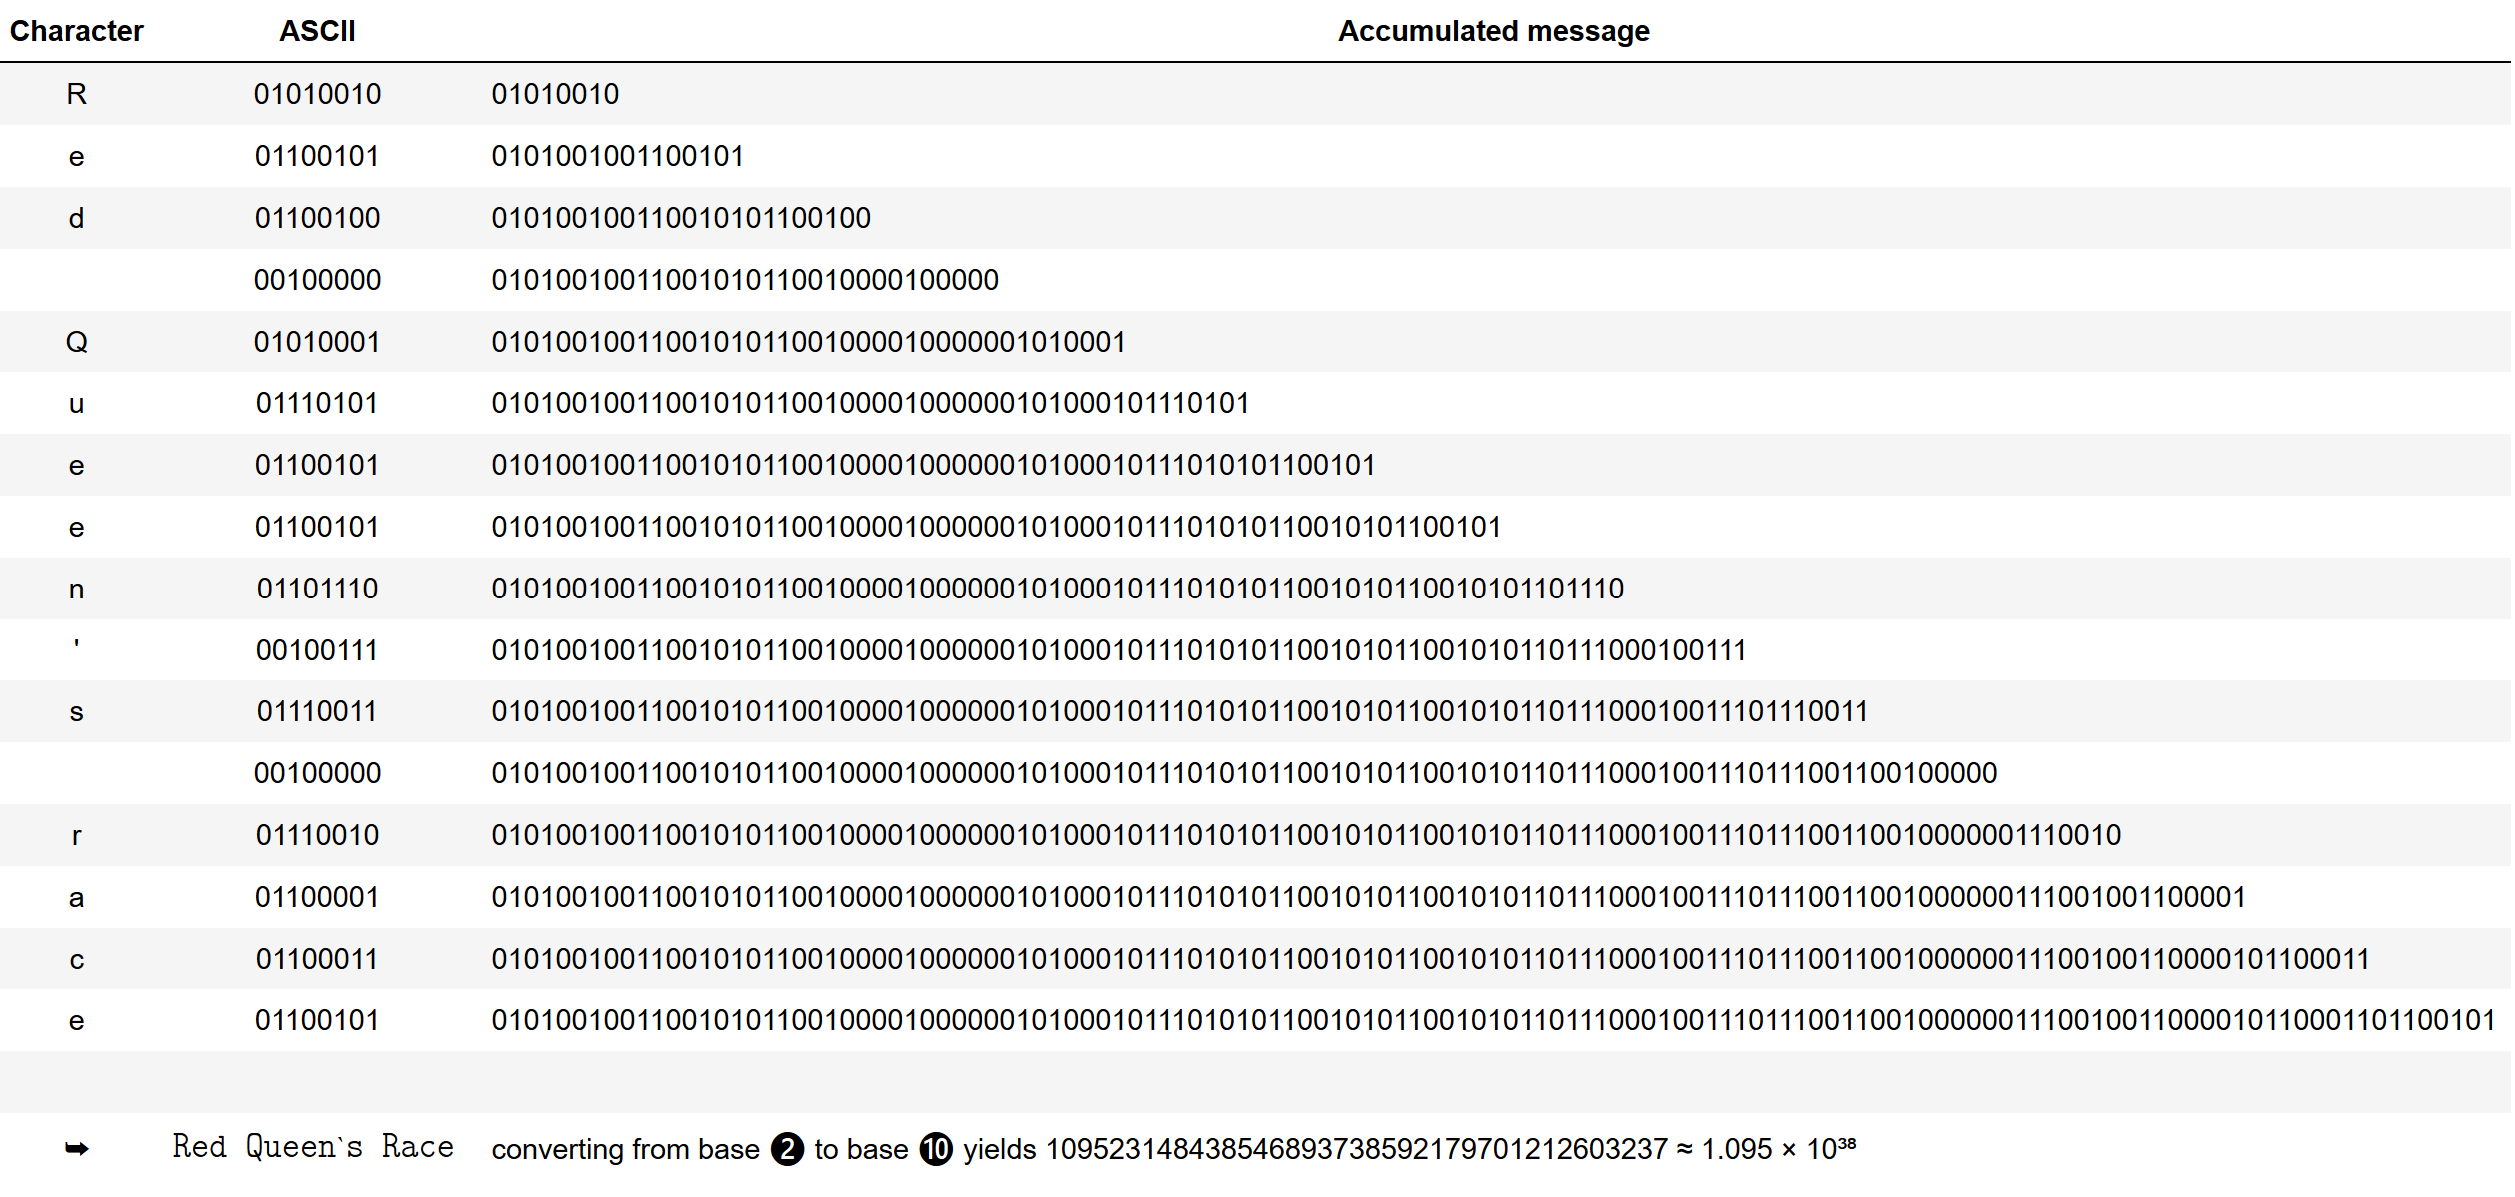
\includegraphics[scale=0.7]{integerTranslation.png}
\caption{Example of how to convert a short message~$\texttt{Red Queen's Race}$ from a sequence of~16 characters into a sequence of~$16 \times 8 = 128$ bits composed of the ASCII codes of all characters appended one after the other.  Once all the characters have been encoded, the final binary string is converted to a decimal number.}
\label{fig:integerTranslation}
\end{figure}

\paragraph{Key generation} The random~$1024$-bit primes~$p$ and~$q$ generated by~\texttt{ssh-keygen} are
\begin{align*}
\hspace*{-1cm} p &= 1652830233930172588028441280420871878125196035749241441410966721827341816066869326344478697902511256  \\
\hspace*{-1cm} & \hspace{0.48cm} 9966686950310590118982385487921794647555777355883884856082484590908509989738447346658862742816573686 \\
\hspace*{-1cm} & \hspace{0.48cm} 3357777495899717471740241145780518183395624614152064709237404036084856914835566384405188943296394177 \\
\hspace*{-1cm} & \hspace{0.48cm} 327957959 \\
\hspace*{-1cm} \big(p &\approx 1.653 \times 10^{308}\big) \\[15pt]
\hspace*{-1cm} q &= 1502597002965083505262633375979403152657038856598614386635166438546449698396221604781928209479169533 \\
\hspace*{-1cm} & \hspace{0.48cm} 8475682032571161153830886284861761570522847010760171950230511297616420536046940575167006542693860665 \\
\hspace*{-1cm} & \hspace{0.48cm} 4576750244537701551043712022710518528333562390395012907956412099441425756277336490106954095150955492 \\
\hspace*{-1cm} & \hspace{0.48cm} 592541789 \\
\hspace*{-1cm} \big(q &\approx 1.503 \times 10^{308}\big)
\end{align*}

\noindent Notice that even though~$p$ and~$q$ are both composed of~$1024$~bits they start to differ at their second decimal digit and therefore the gap~$p - q \approx 1.502 \times 10^{307}$ is so enormous that na\"ive brute-force attacks such as \href{https://en.wikipedia.org/wiki/Fermat\%27s_factorization_method}{Fermat's factorization method} (possible if~$p \approx q$) are automatically ruled out.  Multiplying~$p$ and~$q$ together yields the public modulus~$n = p \cdot q$
\begin{align*}
\hspace*{-1cm} n &= 2483537755913555203879506229460760415936768048414500827933922467152004696505852998792982990321277761 \\
\hspace*{-1cm} & \hspace{0.48cm} 7470542604231099658464774726678493177255047233626637210508539440468877263390150782180405854795055249  \\
\hspace*{-1cm} & \hspace{0.48cm} 6030471354719612929887736729244157142693152362575024781314953697589022772051839077671678244282191782 \\
\hspace*{-1cm} & \hspace{0.48cm} 4291223315475705912822350952049748340648575497655684176841221836101106974492832667442458348194621340 \\
\hspace*{-1cm} & \hspace{0.48cm} 9954408380026753728324536242688309296947434127561960371528514451037596617839124259123219608145478120 \\
\hspace*{-1cm} & \hspace{0.48cm} 1412665154015738765052108165441264356182946222840921843143666861151946253008711697479848139112342071 \\
\hspace*{-1cm} & \hspace{0.48cm} 39252276742648651 \\
\hspace*{-1cm} (n&\approx 2.484 \times 10^{616})
\end{align*}
We see that the expected orders of magnitude~$p \sim q \sim 10^{308}$ and~$n\sim 10^{616}$ determined at the end of section~\ref{sec::algo} for~RSA-2048 are indeed observed here.  Following convention, the public exponent is a relatively small integer given by
\begin{align*}
\hspace*{-7.8cm} e &= 65537 \\
\hspace*{-7.8cm} (e&\approx 6.553 \times 10^{4})
\end{align*}
Euler's totient function~$\varphi(n) = (p-1) \cdot (q-1)$ is evaluated as
\begin{align*}
\hspace*{-1.3cm} \varphi(n) &= 2483537755913555203879506229460760415936768048414500827933922467152004696505852998792982990321277761 \\
\hspace*{-1.3cm} & \hspace{0.48cm} 7470542604231099658464774726678493177255047233626637210508539440468877263390150782180405854795055249  \\
\hspace*{-1.3cm} & \hspace{0.48cm} 6030471354719612929887736729244157142693152362575024781314953697589022772051839077671678244282191782 \\
\hspace*{-1.3cm} & \hspace{0.48cm} 4291223283921433543869790019139001776645825189833335253362663555639775370754917522811549036930552267 \\
\hspace*{-1.3cm} & \hspace{0.48cm} 1786329295603063899507023514555591569111871946775716705087946387907637732589819001269340389886785265 \\
\hspace*{-1.3cm} & \hspace{0.48cm} 0369229974670461360677917937601732671272579105549051797672890689213784897745884986350819393990911686 \\
\hspace*{-1.3cm} & \hspace{0.48cm} 91902606822148904 \\
\hspace*{-1.3cm} \big(\varphi(n) &\approx 2.484 \times 10^{616} \big)
\end{align*}

\noindent Even though~$n$ and~$\varphi(n)$ share more than their first~300 leading digits, they eventually diverge from each other and one can verify that their difference~$n - \varphi(n) = p + q - 1 = 3.155 \times 10^{308}$, though a very large number itself, is completely negligible compared to~$n\sim 10^{616}$.  This should give flesh to the argument made in section~\ref{sec::probaProof} arguing that the probability of a plaintext message not being coprime with the public modulus is infinitesimally small. \\

\noindent The private exponent~$d$ can be efficiently computed using Euclid's extended algorithm as the modular inverse of the public exponent~$e$ with respect to~$\varphi(n)$.  We find
\begin{align*}
\hspace*{-1cm} d &= 8552946755415862940256718433698424185985451707083828018747979016985938630107740998635522848398803589 \\
\hspace*{-1cm} & \hspace{0.48cm} 2138814193126923614378132288803819370835774610213040243095920651140967672416452256559158970157986630  \\
\hspace*{-1cm} & \hspace{0.48cm} 9932975033343250961680610644222443308449341413753804616366099295754191367503854003547580446686462384 \\
\hspace*{-1cm} &  \hspace{0.48cm} 5194761664114432318406573497713851732440647959860594270167282062161791067326622898493471132874950740 \\
\hspace*{-1cm} & \hspace{0.48cm} 8367403482271259320974948612771366055030738336928441343643277839247353956475306293948305934013571483  \\
\hspace*{-1cm} & \hspace{0.48cm} 5716239762014177168698690488071029554392497430801241905103551101752464278518184253465674919873487766 \\
\hspace*{-1cm} & \hspace{0.48cm} 2637011702944913 \\
\hspace*{-1cm} \big( d&\approx 8.553 \times 10^{615} \big)
\end{align*}

\noindent One can explicitly verify that~$e \cdot d \equiv 1 \,\,\text{mod}\,\,\varphi(n)$.  Now that the key generation process is complete, we can move on to the encryption / decryption parts.

\paragraph{Encryption}  The encrypted cipher~$c$ is given by the remainder of division of~$m$ raised to the (rather small) public exponent~$e = 65537$ with the public modulus~$n$
\begin{align*}
\hspace*{-1cm} c &= \mathcal{E}(m) = m^e \,\,\text{mod}\,\,n \\ 
\hspace*{-1cm} & \hspace{0.48cm} 1290081551713542477127470554521689394916224985447577369937337938328332211181590966442841821357849257 \\
\hspace*{-1cm} & \hspace{0.48cm} 7956719649336028503213693001899110981344082059534316812974205798626750761899328504466635981656142944 \\
\hspace*{-1cm} & \hspace{0.48cm} 0270034487934284704529786123974578722296869491128552385351674004877713959958397160178885216967282174  \\
\hspace*{-1cm} & \hspace{0.48cm} 7927924192324256009982344440645602211211412509666911736249710668959360618046546717671884162290977490  \\
\hspace*{-1cm} & \hspace{0.48cm} 3307841867976290293998434632844564867045116909170721515885995688719473914190485526954084354476385592  \\
\hspace*{-1cm} & \hspace{0.48cm} 2383103992959837368412644088564002241028411759208226042349889479042910353430152098596703040208853011  \\
\hspace*{-1cm} & \hspace{0.48cm} 15658025156703529  \\
\hspace*{-1cm} \big( c &\approx 1.29 \times 10^{616} \big)
\end{align*}
which is of the same order of magnitude as the public modulus with~$c \approx 0.52 \, n$.

\paragraph{Decryption}  Operationally, this step is very similar to the encryption in the sense that the original message is recovered by modular exponentiation of the encrypted cipher to the private exponent~$d$ with respect to the public modulus
\begin{align*}
\hspace*{-1cm} \mathcal{D}(c) &= c^d \,\,\text{mod}\,\,n  \\
\hspace*{-1cm}  &= 1070006863906557773181753244912151369846678355638119144582664161559042559075252359660617309043174314 \\
\hspace*{-1cm} & \hspace{0.48cm} 4892790297732870794365932048514840335034219967526428189223919603592270898038626385071086903455682988 \\
\hspace*{-1cm} & \hspace{0.48cm} 9362966321823614168001147021967461629724821385450564072293287067084372107029031933850136051297187681 \\
\hspace*{-1cm} & \hspace{0.48cm} 789299078932638400396786359008268912113436515860008110465019951840714333167627203495615099937 \\
\hspace*{-1cm} &= m
\end{align*}

\noindent Executing~$\mathcal{D}(c)$ na\"ively means that we need to raise a number on the order of~$c \sim 10^{616}$ to another number which is also on the order of~$d \sim 10^{616}$.  Despite the availability of fast modular exponentiation, this operation may become a computational bottleneck. In practice, decryption is split into two dramatically smaller modular exponentiations thanks to the Chinese remainder theorem (CRT).  As shown in~section~\ref{crtOpt}, CRT-optimized decryption reduces the numbers to~$c\,\,\text{mod}\,\,\{p, q\} \lesssim (p, q) \sim (10^{308}, 10^{308})$ and the exponents to~$d \,\,\text{mod}\,\,\{p-1, q-1\} \lesssim (p, q) \sim (10^{308}, 10^{308})$ leading to a speedup of execution by a factor~$\approx 4$ times faster than with the original larger exponent.

\paragraph{\href{https://github.com/Ranlot/public-key-encryption}{Interactive demonstration}} To conclude, we invite the reader to \href{https://github.com/Ranlot/public-key-encryption}{consult the accompanying~\texttt{Jupyter notebook} to run all the steps} described in this example including even more details about CRT-optimization.  In addition to RSA encryption (where the public key is used to encrypt messages and the private key is used for decryption), the notebook also covers the topic of \href{https://en.wikipedia.org/wiki/Digital_signature}{digital signatures} where the private key is used to sign a message thereby allowing recipients to verify the authenticity and integrity of the messages they receive by decrypting the signatures using the public key.

\section{Homomorphisms in textbook RSA}
\label{sec::homomorphisms}

In this section, we show that textbook RSA is a partially homomorphic encryption scheme: it is possible to execute some computations on encrypted ciphertexts which evaluate to the same results (after decryption) as if the same computations had been performed directly on the clear plaintexts.  \\

\noindent Consider two numbers~$m_1$ and~$m_2$ that serve as input to some computation.  If this data is private, we could evaluate the computation ourselves directly on our secure server and collect the private result.  However, our objective is to offload the computational process to some remote unsecure execution environment (cloud server for example) and obtain the correct result without ever revealing anything about~$m_1$ and~$m_2$ or even the result of the computation. Let's start by encrypting~$m_1$ and~$m_2$ with
\begin{align*}
c_1 = \mathcal{E}(m_1) \\
c_2 = \mathcal{E}(m_2)
\end{align*}
where~$\mathcal{E}$ stands for RSA encryption.  These ciphers can now be sent over to the untrusted execution environment.   As far as the recipient of~$c_1$ and~$c_2$ is concerned, all they can see is two random numbers with no way to decrypt or even assign any kind of meaning about what they represent.

\paragraph{Multiplication}  After receiving~$c_1$ and~$c_2$, the server is instructed to multiply them together
\begin{equation*}
c = c_1 \cdot c_2
\end{equation*}
The untrusted server can always evaluate this product and generate a new value~$c$ that appears, as far as it is concerned, to be just as random as the initial input values.  Finally, the server sends~$c$ back to us which we promptly decrypt only to realize that
\begin{equation*}
\mathcal{D}(c) = m_1 \cdot m_2    
\end{equation*}
is precisely the product of the original~$m_1$ and~$m_2$.  To see why this happens, it is enough to realize that the cipher~$c$ can be written as
\begin{align*}
c &= \mathcal{E}(m_1) \cdot \mathcal{E}(m_2) \\
&= \left( m_1^e \,\,\text{mod}\,\,n  \right) \cdot \left( m_2^e \,\,\text{mod}\,\,n  \right) \\
&= \left( m_1 \cdot m_2 \right)^e \,\,\text{mod}\,\,n \\
&= \mathcal{E}(m_1 \cdot m_2)
\end{align*}
In other words, the product of two ciphers is equal to the cipher of the product of the original messages
\begin{equation*}
c = \mathcal{E}(m_1) \cdot \mathcal{E}(m_2) = \mathcal{E}(m_1 \cdot m_2)
\end{equation*}
Applying the RSA decryption function~$\mathcal{D}$ to this cipher shows that:
\begin{equation*}
\mathcal{D}(c) = \mathcal{D} \big( \mathcal{E} (m_1 \cdot m_2 )  \big) = m_1 \cdot m_2
\end{equation*}
In other words, the untrusted execution environment was able to evaluate~$m_1\cdot m_2$ without ever having had any knowledge of~$m_1, m_2$ and even of the result since all it ever was exposed to were the encrypted ciphers~$c_1, c_2$ and~$c$.

\paragraph{Division}  Let us now assume that we want to compute the division~$m_1 / m_2$.  For simplicity, we restrict ourselves to situations for which~$m_2$ divides $m_1$ so that the result of~$m_1 / m_2$ remains in the set of integers.  Assuming that~$m_2$ and the modulus~$n$ are coprimes, one can efficiently determine the modular inverse~$m^{-1}_{2 \, \%n}$ of~$m_2$ that satisfies
\begin{equation*}
m_2 \cdot m^{-1}_{2 \, \%n} \equiv 1 \,\,\text{mod}\,\,n
\end{equation*}
and the division~$m_1 / m_2$ can be replaced by a multiplication~$m_1 \cdot m^{-1}_{2 \, \%n}$ which we have already shown to be preserved under textbook RSA encryption in the paragraph above.

\paragraph{Addition/Subtraction}  Unfortunately, these operations cannot be evaluated homomorphically since
\begin{equation*}
\mathcal{E}(m_1) + \mathcal{E}(m_2) \neq \mathcal{E}(m_1 + m_2)
\end{equation*}

\section{Real-world RSA: randomized padding~\textemdash~OAEP}
\label{sec::padding}

\noindent So far, our description of RSA has been limited to what is usually referred to as ``textbook'' RSA.  Because of its crucial importance to digital communication, the algorithm has been the subject of intense research and a large number of attacks are well-documented. Some attacks exploit implementation weaknesses (for example, insufficient randomness in IoT devices~\cite{randomness} causes pseudorandom numbers to rapidly start repeating themselves thereby dramatically reducing the search space to such a small size that trivial collisions as described in section~\ref{sec::algo} become realistic). Others exploit inherent issues associated with \href{https://en.wikipedia.org/wiki/Coppersmith\%27s_attack#H\%C3\%A5stad's_broadcast_attack}{mass broadcasts of the same message encrypted with different public keys}. Even more sophisticated side-channel attacks (such as timing~\cite{sideChannel:timing} or even acoustic cryptanalysis~\cite{sideChannel:acoustics}...) are also possible.  In addition to many more incredibly creative attack vectors~\cite{boneh}, textbook RSA suffers from other conceptual flaws as far as security is concerned.

\subsection{Some conceptual issues with ``textbook'' RSA...}

\paragraph{Malleability}  Because of the homomorphisms described in section~\ref{sec::homomorphisms}, it is possible for an attacker to modify ciphers in a controlled way that has a predictable impact on the content of the messages.  Although homomorphisms are clearly useful for computing on encrypted data, the malleability they introduce into a cryptosystem can also be considered an undesirable property from a security perspective as it may be exploited for nefarious purposes~\footnote{To see an extreme example of how malleability can be exploited, we refer the reader to the \href{https://github.com/Ranlot/public-key-encryption}{notebook dedicated to the ``one-time pad''} where the level of resolution one can achieve is even more fine-grained in the context of stream ciphers.}. A well-known attack vector based on malleability is known as Chosen Cipertext Attacks~\textemdash~CCAs. Let's image a resourceful adversary that is able to obtain the decryptions of certain chosen ciphertexts.  Because of RSA malleability, they can use this information to recover secret messages. For example, the attacker could intercept a cipher~$c = \mathcal{E}(m)$ which encrypts a secret message~$m$ and use it to create a new cipher~$c_\text{attack} = c \times \mathcal{E}(r)$ where the attacker multiplied the original cipher with the encryption of a plaintext~$r$ of their choosing (using the public key).  Due to the multiplicative homomorphicity of RSA, the attacker also knows that~$\mathcal{D}(c_\text{attack}) \equiv m \times r \,\,\text{mod}\,\,n$ and, assuming that they were able to obtain~$\mathcal{D}(c_\text{attack})$, extracting~$m$ becomes trivial. 

\paragraph{Lack of semantic security}  Ideally one would like cryptosystems to be such that ciphers reveal nothing about the messages.  In other words, seeing a ciphertext should not let the adversary be able to guess anything about the message with a better chance of success than if they had not seen the ciphertext; a concept known as ``perfect secrecy''~\footnote{See the \href{https://github.com/Ranlot/public-key-encryption}{notebook dedicated to the ``one-time pad'' in order to see a demonstration of perfect secrecy}.}. Obviously, as a deterministic algorithm, this is not a property of textbook RSA.  For example, an adversary could prepare a list of messages ahead of time and compare their ciphers (encrypted with the public key) with an intercepted cipher to look for matches; a process known as Chosen Plaintext Attacks~\textemdash~CPAs.  Similarly, although observing twice the same cipher does not tell an attacker what the message is, it does nonethless reveal the fact that the same message was sent twice. \\

\noindent The solution adopted to remedy these issues is to introduce some randomization in the form of a padding scheme known as Optimal Asymmetric Encryption Padding~\textemdash~OAEP.  Despite the existence of numerous pitfalls that require paying great attention to details, successful implementations of RSA~+~OAEP can be trusted to provide high-level of security and no devastating attacks have ever been found so far. It should also be clear that RSA~+~OAEP no longer has any homomorphic properties.

\subsection{Optimal Asymmetric Encryption Padding~\textemdash~OAEP}  

Let us add a few pointers to help read the logic of~OAEP illustrated in~Figure~\ref{fig:oaep}.  The random seed consists of~20 bytes typically collected from \texttt{/dev/random/} or from a pseudorandom number generator. For security reasons that go beyond the scope of this tutorial, it is necessary to allocate another~20~bytes of the data block to a hashed label.  In the context of~OAEP, a simple SHA1 hash of the empty string \\

\noindent \verb$SHA1("") = \xda9\xa3\xee^kK\r2U\xbf\xef\x95`\x18\x90\xaf\xd8\x07\t$ \\

\noindent is usually considered good enough for real-world implementations. Overall, OAEP overhead leaves us with~214~bytes with which to encode plaintext messages.  Assuming that each byte represents an ASCII character, this translates into a~214-character limit before messages need to be chunked.

\newpage

\begin{figure}[t]
\centering
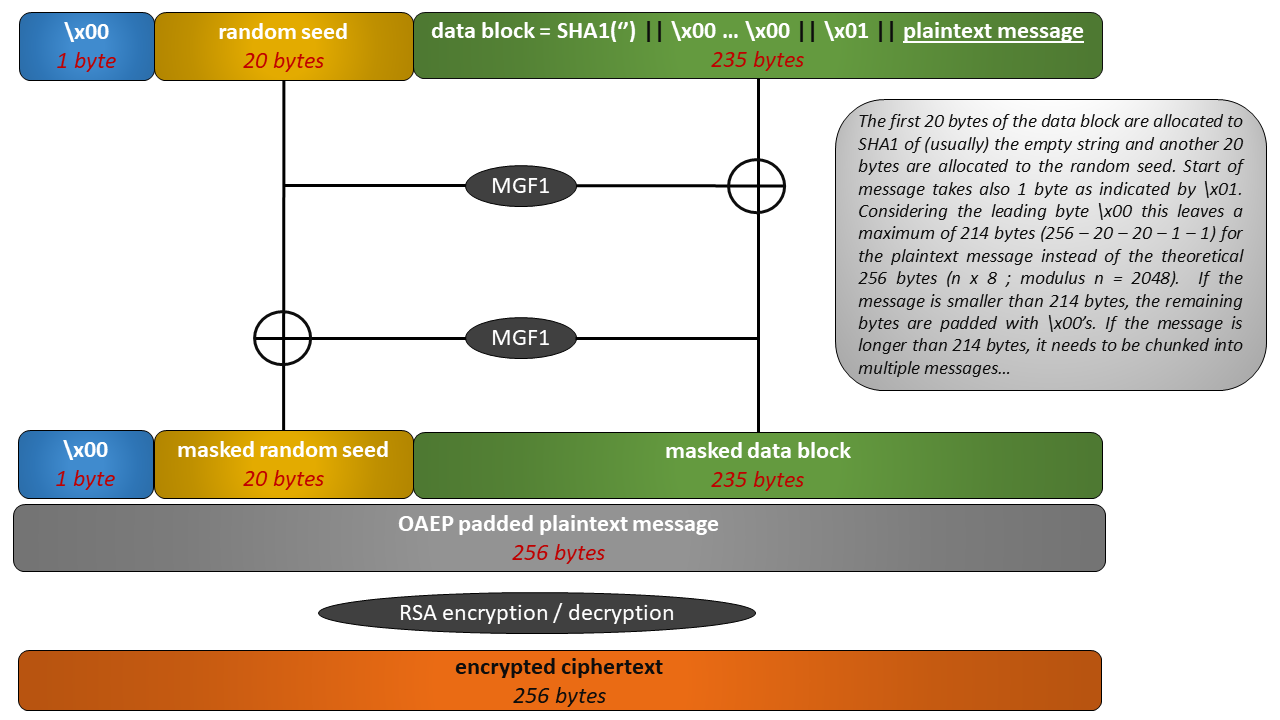
\includegraphics[scale=0.46]{oaep.png}
\caption{The padding scheme has a completely reversible structure: reading from {\bf top to bottom} corresponds to OAEP padding~+~encryption whereas reading from the {\bf bottom up} characterizes OAEP unpadding~+~decryption.  Unsuprisingly, the XOR-looking symbols~$\oplus$ indeed correspond to logical~XOR operations between the incoming sequences of bits. MGF1 is an instance of \href{https://en.wikipedia.org/wiki/Mask_generation_function}{Mask Generation Functions}.  These functions provide similar functionality to hash functions but are more general since they can generate (deterministic) output of any user-specified length. In our case, we use~MGF1 to take in 20 bytes (resp. 235 bytes) and hash them to 235 bytes (resp. 20 bytes).}
\label{fig:oaep}
\end{figure}

\paragraph{Padding} We start by expanding the~20-byte random seed~$r$ into another pseudorandom~235~byte-long hash~$\text{MGF1}(r)$ using the~\href{https://en.wikipedia.org/wiki/Mask_generation_function}{MGF1 Mask Generation Function}.  Next, the~data block~$\text{db}$ is masked into a randomized data block~$\text{db}_m = \text{db} \oplus \text{MGF1}(r)$.  Finally, the random seed~$r$ itself is also masked by combining it with a MGF1 hash of~$\text{db}_m$ from its original~235~bytes down to~20~bytes with~$r_m = r \oplus \text{MGF1}(\text{db}_m)$.  Concatenating together the masked random seed~$r_m$ and the masked data block~$\text{db}_m$ defines a randomized version of our original plaintext which is now padded such that it always contains the full~$256$ bytes possible in RSA-2048.

\paragraph{Unpadding} Going back from the encrypted cipher to the original plaintext is a completely symmetric process which reverses all the steps carried out during the padding procedure.  Clearly, we start by using the RSA private key to go from the encrypted cipher to the random padded plaintext.  At this point, the message has been decrypted and all that is left is a parsing problem to revert the random padding and extract the original plaintext.  We know that the first~20~bytes (after parsing out the initial~\verb$\x00$ byte) consist of the masked random seed~$r_m$ and that the remaining~235~bytes can be identified with the masked data block~$\text{db}_m$.  Following~Figure~\ref{fig:oaep} from bottom to top shows that the random seed~$r$ can be recovered by evaluating~$r_m \oplus \text{MGF1} ( \text{db}_m) \rightarrow r$~\footnote{The masked random seed was originally defined as~$r_m = r \oplus \text{MGF1}(\text{db}_m)$ during the padding procedure. Therefore:
\begin{equation*}
r_m \oplus \text{MGF1} ( \text{db}_m)  =  r \oplus \text{MGF1}(\text{db}_m) \oplus \text{MGF1}(\text{db}_m) = r    
\end{equation*}
}.  Now that~$r$ is known, the data block~$\text{db}$ can be recovered by evaluating~$\text{db}_m \oplus \text{MGF1}(r) \rightarrow \text{db}$~\footnote{Once again, this is because the masked data block was originally defined as~$\text{db}_m = \text{db} \oplus \text{MGF1}(r)$.  Therefore:
\begin{equation*}
\text{db}_m \oplus \text{MGF1}(r) =  \text{db} \oplus \text{MGF1}(r) \oplus \text{MGF1}(r) = \text{db}
\end{equation*}
}.  After verifying that the first~20~bytes correspond to the expected~\verb$SHA1("")$ bit sequence, one looks for the first occurrence of~\verb$\x01$ in order to know where the original plaintext message actually starts and the OAEP unpadding is complete. 

\section{Technical background}

\noindent The purpose here is just to gather some useful and well-known results disguised as pseudo-``theorems'' for which serious proofs and discussions can easily be found online.

\begin{theorem} \href{https://en.wikipedia.org/wiki/Extended_Euclidean_algorithm}{\hypertarget{theorem1}{Euclid's extended algorithm}} is an efficient procedure that simultaneously yields the greatest common divisor~$\text{gcd}(a,b)$ of two numbers~$a$ and~$b$ in addition to the coefficients~$a^{-1}_{\%b}$ and~$b^{-1}_{\%b}$ of the B\'ezout's identity
\begin{equation*}
\text{gcd} (a, b)  =  a \cdot a^{-1}_{\%b} + b \cdot b^{-1}_{\%a}
\end{equation*}
The notation makes sense when one considers the (common for our purposes) situation in which~$a$ and~$b$ are coprimes.  In this case, the greatest common divisor is~$\text{gcd}(a, b) = 1$ and the following identities hold
\begin{equation*}
1 = a \cdot a^{-1}_{\%b} + b \cdot b^{-1}_{\%a}  \quad \rightarrow \quad \begin{pmatrix}
a \cdot a^{-1}_{\%b} \equiv 1 \,\,\text{mod}\,\,b \\[0.3em]
b \cdot b^{-1}_{\%a} \equiv 1 \,\,\text{mod}\,\,a
\end{pmatrix}
\end{equation*}
revealing that~$a^{-1}_{\%b}$ is the modular inverse of~$a$ in~$\mathbb{Z}_b$ and that~$b^{-1}_{\%a}$ is the modular inverse of~$b$ in~$\mathbb{Z}_a$.
\end{theorem}

\begin{theorem}
(\href{https://en.wikipedia.org/wiki/Fermat\%27s_little_theorem}{\hypertarget{theorem2}{Fermat's little theorem}}) Given a prime number~$p$ and an integer~$a$ so that~$p$ does not divide~$a$
\begin{equation*}
a^{p-1} \equiv 1 \,\,\text{mod}\,\, p
\end{equation*}
\end{theorem}
This theorem can be used as a simple probabilistic test for primality of~$p$ by picking a few random integers~$a$ not divisible by~$p$ and seeing whether the equality holds.  If it does then~$p$ is probably prime.

\begin{theorem}
(\href{https://en.wikipedia.org/wiki/Euler\%27s_theorem}{\hypertarget{theorem3}{Euler's theorem}}) Given two integers~$a$ and~$n$ coprime with each other i.e.\ $\text{gcd}(a,n)=1$ and \href{https://en.wikipedia.org/wiki/Euler\%27s_totient_function}{Euler's totient function}~$\varphi$, we have
\begin{equation*}
a^{\varphi(n)} \equiv 1 \,\,\text{mod}\,\,n
\end{equation*}
\end{theorem}
This is a generalization of Fermat's little theorem that covers cases when~$n$ is composite. In the special case where~$n$ is prime~$\varphi(n) = n-1$ and the congruence immediately reduces to Fermat's little theorem.

\begin{theorem}
\hypertarget{theorem4}{Given} a prime~$p$ and two positive integers~$a, k$, then 
\begin{equation*}
a^k \equiv a^{k \,\,\text{mod}\,\,p-1} \,\,\text{mod}\,\, p
\end{equation*}
\end{theorem}
This theorem is useful to reduce the magnitude of the exponent during modular exponentiation.  Note that this is valid for all~$a$ and~$k$ without any coprimality restrictions as long as~$p$ is a prime number. \\

\noindent In order to see why this is true, it is useful to consider two branches depending on whether the prime~$p$ divides~$a$ or not
\begin{itemize}
\item $p$ does not divide~$a$. Using Euclidean division of~$k$ with~$p-1$, it is always possible to write the exponent as~$k = q(p-1) + r$ with a remainder~$r \equiv k \,\,\text{mod}\,\,p-1$.  Applying Fermat's little theorem~$a^{p-1}\equiv 1\,\,\text{mod}\,\,p$ in the evaluation of~$a^k$ leads to
\begin{align*}
a^k &\equiv a^{q(p-1) + r} \,\,\text{mod}\,\, p \\
&\equiv \underbrace{\big( a^{p-1} \times \cdots \times a^{p-1} \big)}_{q \, \text{times}} \, \times \, a^r  \,\,\text{mod}\,\, p \\
&\equiv a^r \,\,\text{mod}\,\, p \\
&\equiv a^{k \,\,\text{mod}\,\,p-1} \,\,\text{mod}\,\, p
\end{align*}
\item $p$ divides~$a$. In this case,~$a$ can be expressed as a multiple of~$p$.  As a result, raising~$a$ to {\bf any power} will always lead to another integer that is necessarily also a multiple of~$p$.  Therefore, both sides of the congruence~$a^k \,\,\text{mod}\,\, p$ and~$a^{k \,\,\text{mod}\,\,p-1} \,\,\text{mod}\,\, p$ evaluate to~$0$ and the original statement
\begin{equation*}
a^k \equiv a^{k \,\,\text{mod}\,\, p-1} \,\,\text{mod}\,\, p \quad \quad \text{reduces to} \quad \quad 0 \equiv 0 \,\,\text{mod}\,\, p \quad \quad \text{which trivially holds.}
\end{equation*}
\end{itemize}

\begin{theorem}
(\href{https://en.wikipedia.org/wiki/Chinese_remainder_theorem}{\hypertarget{theorem5}{Chinese remainder theorem}}~\textemdash~CRT) Let~$p$ and~$q$ be coprimes.  The system of congruences
\begin{equation*}
\begin{pmatrix}
x \equiv a \,\,\text{mod}\,\, p \, \in \mathbb{Z}_p \\
x \equiv b \,\,\text{mod}\,\, q \, \in \mathbb{Z}_q
\end{pmatrix} \,\, \text{has a unique solution in } \mathbb{Z}_{pq} \,\,\, \text{given by} \,\,\, x \equiv \big( b p p^{-1}_{\%q} + a q q^{-1}_{\%p} \big) \,\,\text{mod}\,\,pq
\end{equation*}
where the modular inverses~$p^{-1}_{\%q}$ and~$q^{-1}_{\%p}$ can be found via Euclid's extended algorithm.  Equivalently, any integer~$x \in \mathbb{Z}_{pq}$ (where~$p$ and~$q$ are coprime with each other) can be uniquely decomposed in the cartesian product~$\mathbb{Z}_p \times \mathbb{Z}_q$
\begin{equation*}
x \in \mathbb{Z}_{pq} \,\, \Longleftrightarrow \,\, 
\begin{pmatrix}
a \equiv x \,\,\text{mod}\,\, p \, \in \mathbb{Z}_p \\
b \equiv x \,\,\text{mod}\,\, q \, \in \mathbb{Z}_q
\end{pmatrix}
\end{equation*}
\end{theorem}

\noindent It is easy to verify that the proposed solution~$x$ in the theorem indeed satisfies the system of congruences
\begin{equation*}
\begin{pmatrix}
x \,\,\text{mod}\,\, p  \\[0.3em]
x \,\,\text{mod}\,\, q
\end{pmatrix}
\equiv
\begin{pmatrix}
a q q^{-1}_{\%p} \,\,\text{mod}\,\,p \\[0.3em]
b p p^{-1}_{\%q} \,\,\text{mod}\,\,q
\end{pmatrix}
\equiv
\begin{pmatrix}
a \,\,\text{mod}\,\,p \\[0.3em]
b \,\,\text{mod}\,\,q
\end{pmatrix}
\end{equation*}
where we used B\'ezout's identity with~$\text{gcd}(p, q)=1$ along with the properties of the modular inverses~$p^{-1}_{\%q}$ and~$q^{-1}_{\%p}$ discussed in Theorem~1.

\paragraph{Slight rewriting} Note that the solution~$x$ can be rewritten using B\'ezout's identity as
\begin{equation*}
x \equiv \big( b p p^{-1}_{\%q} + a q q^{-1}_{\%p} \big) \,\,\text{mod}\,\, pq \,\,\, \Longleftrightarrow \,\,\, x\equiv \big( b + q q^{-1}_{\%p} (a - b) \big) \,\,\text{mod}\,\, pq
\end{equation*}
This way, only a single modular inverse~$q^{-1}_{\%p}$ needs to be kept in memory when decrypting ciphers as is actually implemented in~\texttt{ssh-keygen} (see \href{https://github.com/Ranlot/public-key-encryption}{accompanying~\texttt{Jupyter notebook}}).

\paragraph{Special case of the theorem}  Let's consider the special case where~$a = b$.  If an integer~$x$ satisfies two identical congruence relations
\begin{equation*}
\begin{pmatrix}
x \equiv a \,\,\text{mod}\,\,p \\
x \equiv a \,\,\text{mod}\,\,q
\end{pmatrix} \quad \text{then the solution reduces to} \quad x \equiv a \,\,\text{mod}\,\, pq    
\end{equation*}


\begin{thebibliography}{10}

\bibitem{rsaOriginal} Ron Rivest, Adi Shamir \& Leonard Adleman. \href{https://people.csail.mit.edu/rivest/Rsapaper.pdf}{``A Method for Obtaining Digital Signatures and Public-Key Cryptosystems''}. (1978) (MIT)

\bibitem{RSAquantum} Riccardo Mengoni, Daniele Ottaviani \& Paolino Iorio. \href{https://arxiv.org/pdf/2005.02268.pdf}{``Breaking RSA Security With A Low Noise D-Wave 2000Q Quantum Annealer: Computational Times, Limitations And Prospects''} (2020)

\bibitem{sigmaprime} Kristian Mcdonald. \href{https://blog.sigmaprime.io/introduction-to-rsa.html}{``A Detailed Introduction to RSA Cryptography''}. Sigma Prime

\bibitem{Harvey} David Harvey \& Joris van der Hoeven \href{https://hal.archives-ouvertes.fr/hal-02070778/document}{``Integer multiplication in time $O(n \log n)$''}. (2019) (\'Ecole Polytechnique \& University of New South Wales) 

\bibitem{randomness} JD Kigallin. \href{https://info.keyfactor.com/factoring-rsa-keys-in-the-iot-era}{``The Irony (and Dangers) of Predictable Randomness''}

\bibitem{sideChannel:timing} Paul C. Kocher. \href{https://www.paulkocher.com/doc/TimingAttacks.pdf}{``Timing Attacks on Implementations of Diffie-Hellman, RSA, DSS and Other Systems''}. CRYPTO 1996 

\bibitem{sideChannel:acoustics} Daniel Genkin, Adi Shamir \& Eran Tromer. \href{https://www.cs.tau.ac.il/~tromer/papers/acoustic-20131218.pdf}{``RSA Key Extraction via Low-Bandwidth Acoustic Cryptanalysis''}. CRYPTO 2014 (Technion, Tel Aviv University \& Weizmann Insitute of Science)

\bibitem{boneh} Dan Boneh. \href{http://www.ams.org/notices/199902/boneh.pdf}{``Twenty Years of Attacks on the RSA Cryptosystem''}. Notices of the AMS (1999) (Stanford)



\end{thebibliography}

\end{document}
